\chapter{Background and Preliminaries}
\label{chap:Background}
\section{Block Diagram}
\begin{figure}[h!]
    \centering
    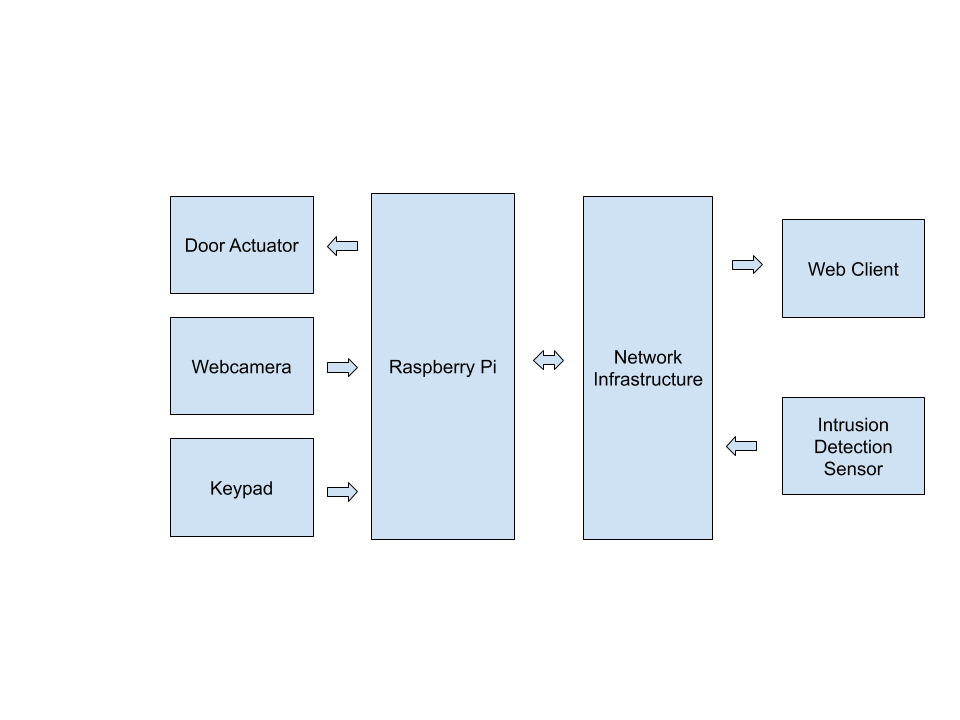
\includegraphics[width=13cm]{images/functional_block_diagram.png}
    \caption{Block Diagram of Facial Recognition Based Entry Logging and Intrusion Detection}
\end{figure}

\begin{flushleft}
    The proposed system is a combination of interrupt based signal from the sensors and pooling based data from the 
    camera. The block diagram shows how the Raspberry Pi can communicate with the various part of the the system. 
    The intrusion detection sensors are connected by wireless means with the Raspberry Pi. The Networking Infrastructure
    exposes the Raspberry Pi to the outside world through a secure channel.
\end{flushleft}

\section{Flow Chart}
\begin{figure}[h!]
    \centering
    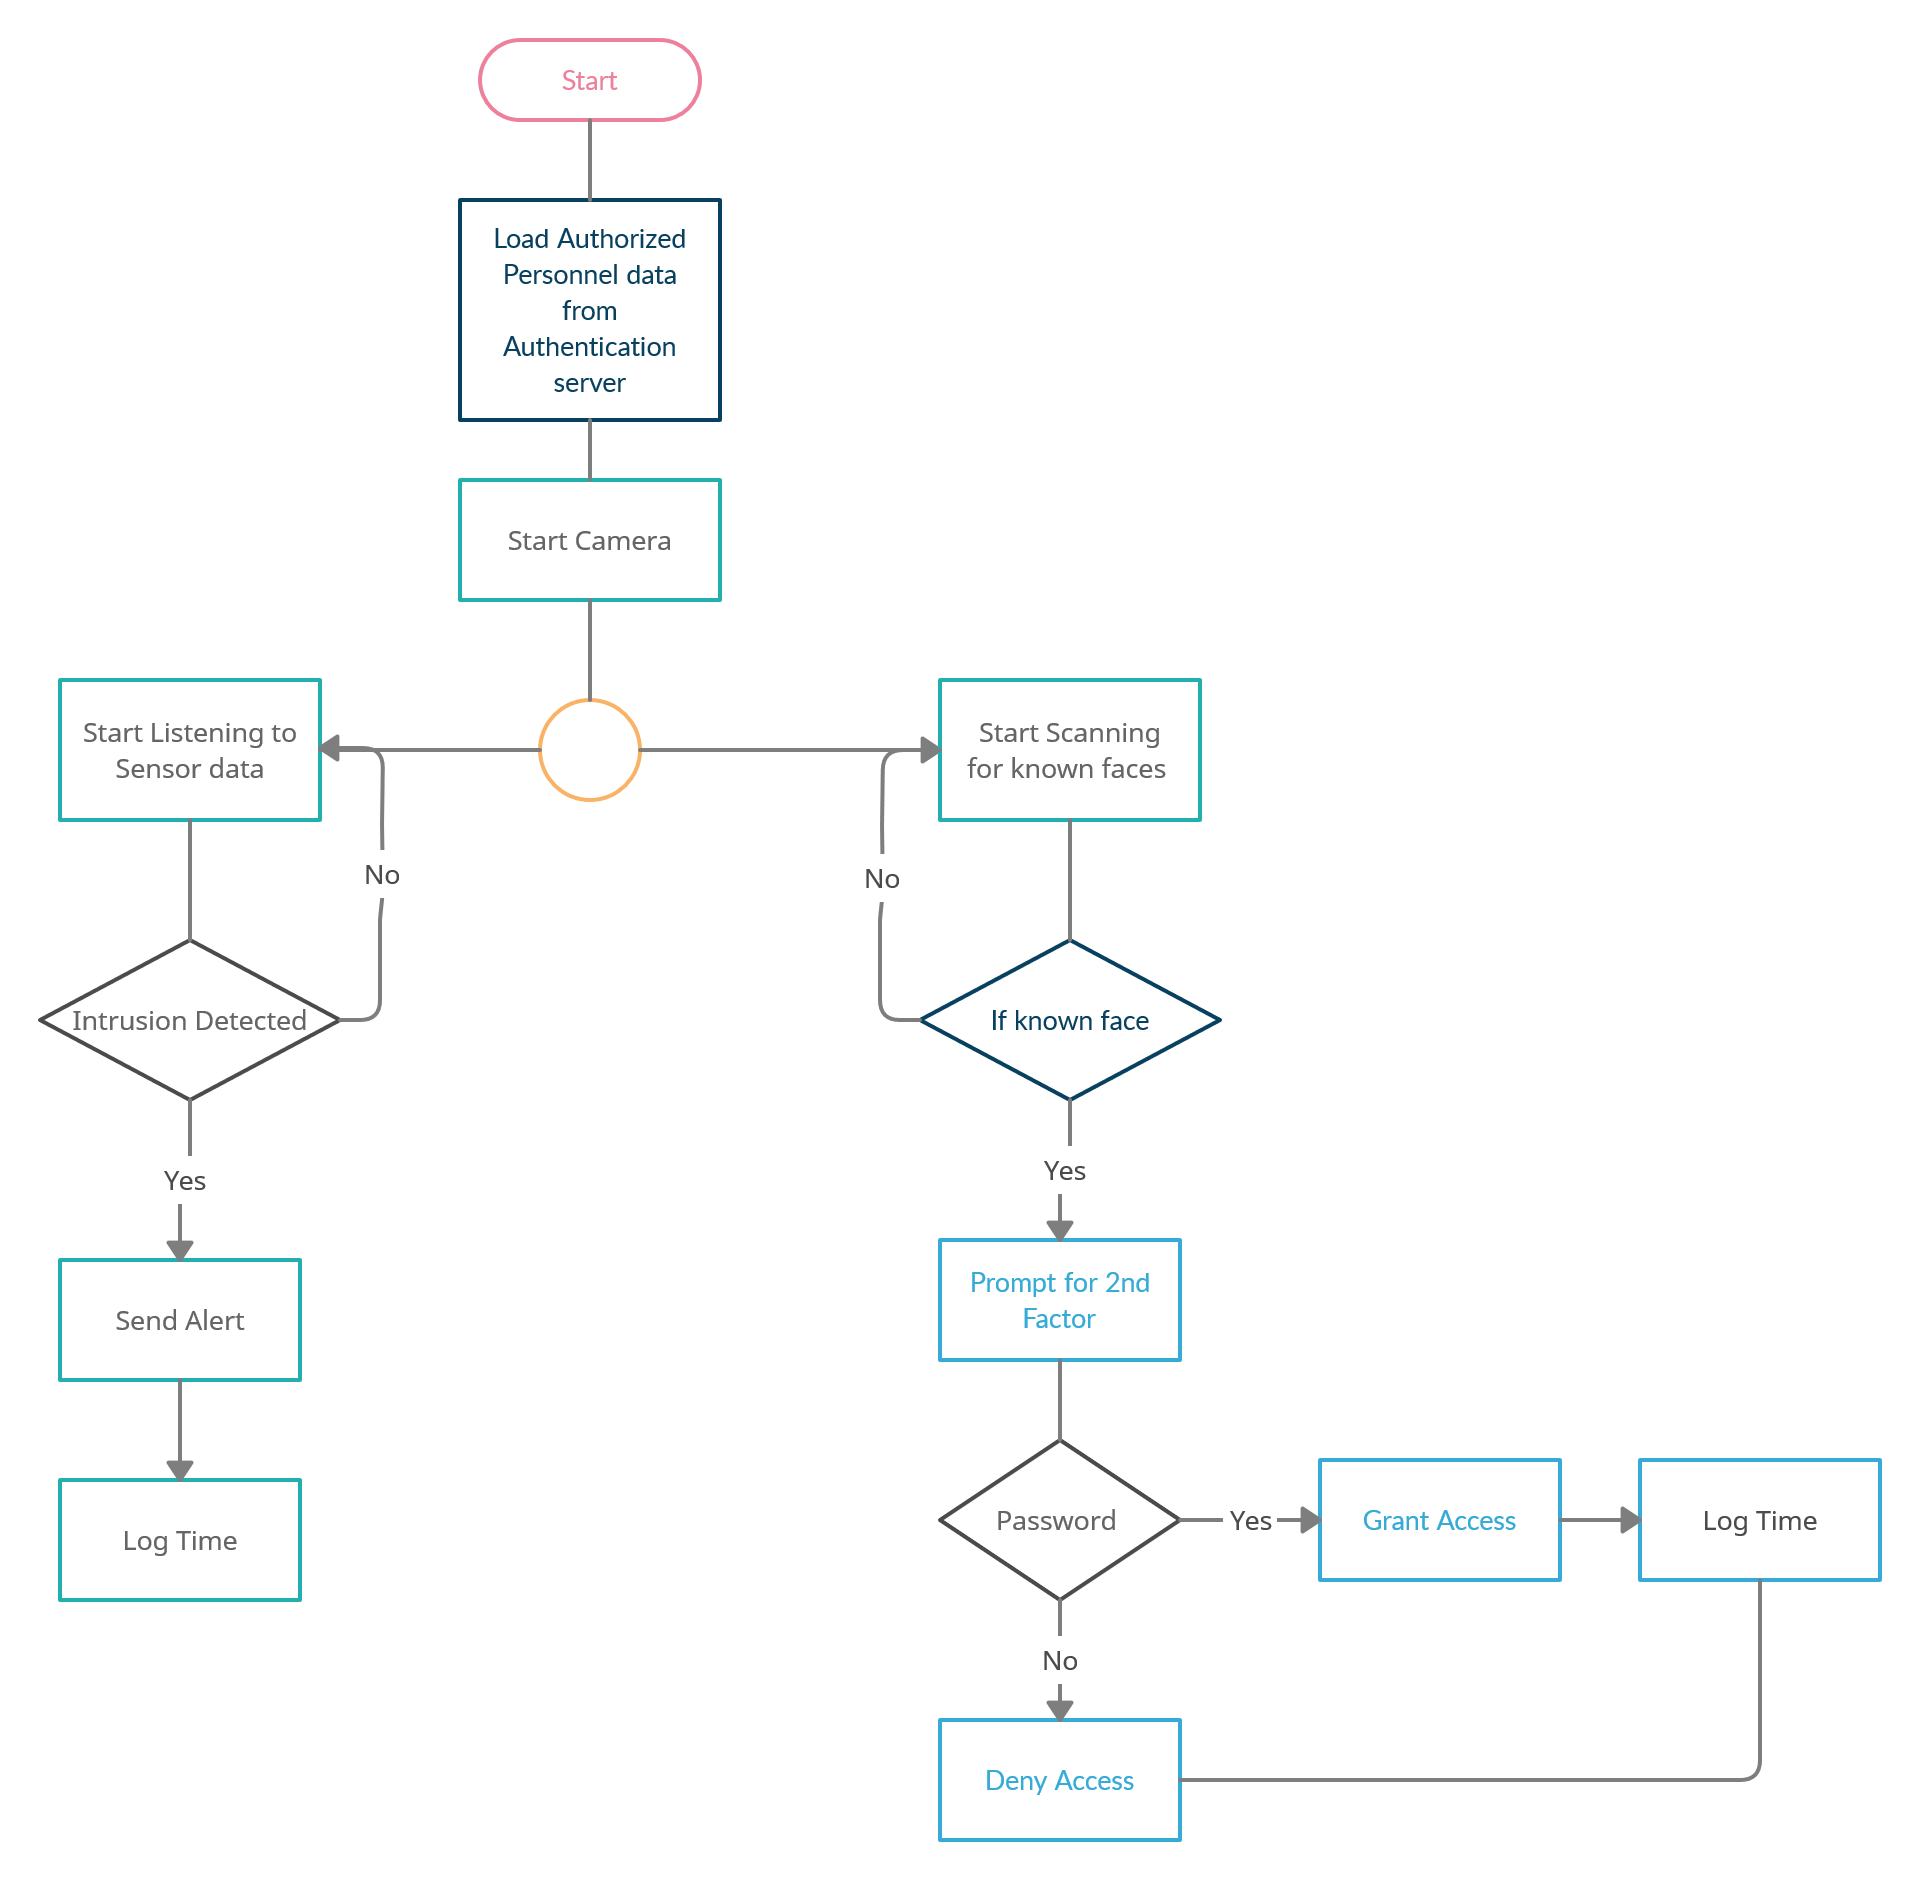
\includegraphics[width=14cm]{images/flowchart.png}
    \caption{Flow Chart of Facial Recognition Based Entry Logging and Intrusion Detection}
\end{figure}


\section{Required Components}
\begin{enumerate}
    \item Raspberry Pi 3B(x1)
    \item Micro SD Card (x1)
    \item Web camera (x1)
    \item Keypad (x1)
    \item ESP8266 (x1)
    \item Magnetic Contact switch (x1)
    \item WiFi Router (x1)
    \item Power Adapter [5V-2A] (x2)
    \item Wires
\end{enumerate}

\section{Description of Components}

    \subsection{Raspberry Pi 3B}
        \begin{figure}[H]
            \centering
            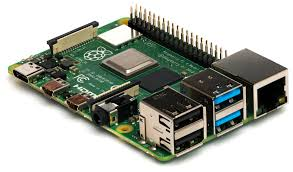
\includegraphics[width=6cm]{images/rpi.jpg}
            \caption{Raspberry Pi 3B+}
        \end{figure}

        \begin{flushleft}
            Raspberry Pi is the worlds first small single board computer. It has invented the form factor that it still dominates. 
            This small computer has a ARM CPU and GPU with on board robust Networking, the board is also very low power consuming. 
            These characteristics make this board the perfect choice for home Automation and IOT based projects.
        \end{flushleft}
        \textbf{Specification: }
        \begin{itemize}
            \item CPU Clock Speed: 1.2GHz
            \item RAM: 1GB
            \item WiFi: 2.4GHz
            \item GPIO: 40pins
            \item Power: 20W
            \item USB: 4x USB 2.0
        \end{itemize}

    \subsection{Micro SD Card}
        \begin{figure}[H]
            \centering
            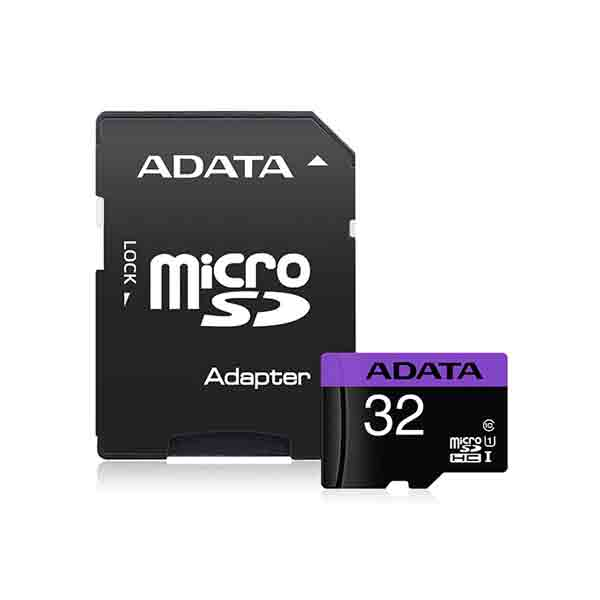
\includegraphics[width=4cm]{images/sdcard.jpg}
            \caption{Micro SD Card}
        \end{figure}
        \begin{flushleft}
            Micro SD card is another modern marvel of technology. It's one of the smallest and most reliable data storage  medium. 
            For running a Operating system in the Raspberry Pi, we need to boot from the SD card.
        \end{flushleft}
        \textbf{Specification: }
        \begin{itemize}
            \item Dimensions: $15*11*1$mm
            \item Speed Class: 10
            \item Seq. Write: 10MB/s
            \item Seq. Read: 15MB/s
        \end{itemize}


    \subsection{Web Camera}
        \begin{figure}[H]
            \centering
            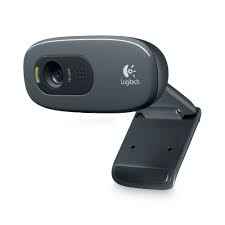
\includegraphics[width=5cm]{images/webcam.jpg}
            \caption{USB Web Camera}
        \end{figure}
        \begin{flushleft}
            A web camera is essentially a USB camera that can be connected to any computer including the Raspberry Pi. In our project 
            this camera will be used to detect the facial features of the users face.
        \end{flushleft}
        \textbf{Specification: }
        \begin{itemize}
            \item Resolution: 720p
            \item USB: USB 3.0
            \item Focus: Infinite/Fixed
            \item Mic: Yes 
            \item Framerate: 30FPS
            \item FOV: 60$\circ$
        \end{itemize}

    \subsection{Keypad}
        \begin{figure}[H]
            \centering
            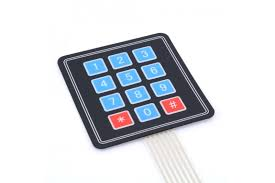
\includegraphics[width=4cm]{images/keypad.jpg}
            \caption{Keypad}
        \end{figure}
        \begin{flushleft}
            Keypad can be used to input password to the device. It's a cheap and effective input device. Other than taking the input from the user, 
            this same keyboard can be used to configure the device when first setting up.
        \end{flushleft}
        
        \textbf{Specification: }
        \begin{itemize}
            \item Matrix Config: 4X4
            \item Max Voltage: 24V
            \item Max Current: 30mA
            \item Very thin 
            \item Adhesive backing
            \item Operating Temperature: 0C to 50C
        \end{itemize}
        
    \subsection{ESP8266}
        \begin{figure}[H]
            \centering
            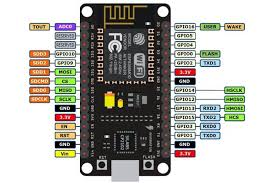
\includegraphics[width=5cm]{images/esp.jpg}
            \caption{ESP8266}
        \end{figure}
        \begin{flushleft}
            A single board micro controller board with on board WiFi capabilities and very low power consumption. Being a micro controller it has
            very good interface potential and robust connectivity/expandability. 
        \end{flushleft}

        \textbf{Specification:}
            \begin{itemize}
                \item Wi-fi: 802.11 b/g/n, Wi-Fi Direct, soft-AP
                \item Flash: 4MB
                \item CPU: 80MHz
                \item Standby power: 1.0mW
            \end{itemize}

    \subsection{Magnetic Contact Switch}
        \begin{figure}[H]
            \centering
            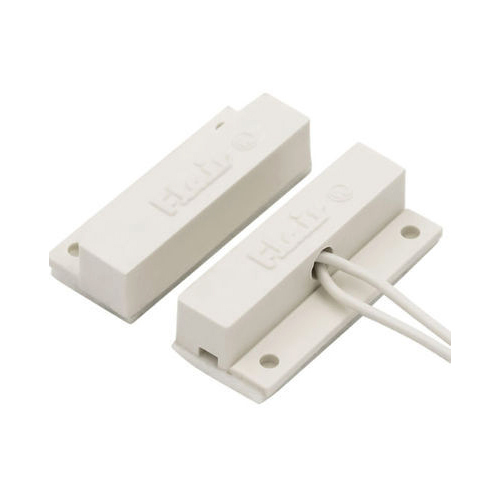
\includegraphics[width=3cm]{images/switch.jpg}
            \caption{Magnetic Contact Switch}
        \end{figure}

        \begin{flushleft}
            A switch that closes contacts when magnets are moved away from the device. This will be responsible for waking up the micro controller 
            and sending the signal.
        \end{flushleft}

   \subsection{Wi-Fi Router}
   \begin{figure}[H]
       \centering
       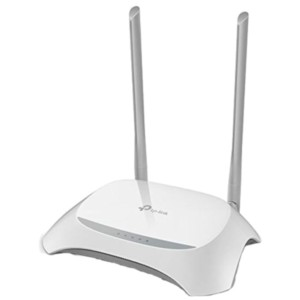
\includegraphics[width=3cm]{images/router.jpg}
       \caption{Wi-Fi Router}
   \end{figure}

   \begin{flushleft}
       Router will be the central part of the Networking Infrastructure. This router will connect the devices internally then will be used 
       to interface with the internet. The firewall on the router will be responsible for securing it from outside threat. 
   \end{flushleft}
   \textbf{Specification:}
   \begin{itemize}
       \item Wi-Fi: 2.4GHz
       \item Mode: 802.11 b/g/n
       \item Channel: 11
       \item Power: 20W
       \item Uplink: 100Mbps
   \end{itemize}

    \subsection{Power Adapter}
        \begin{figure}[H]
            \centering
            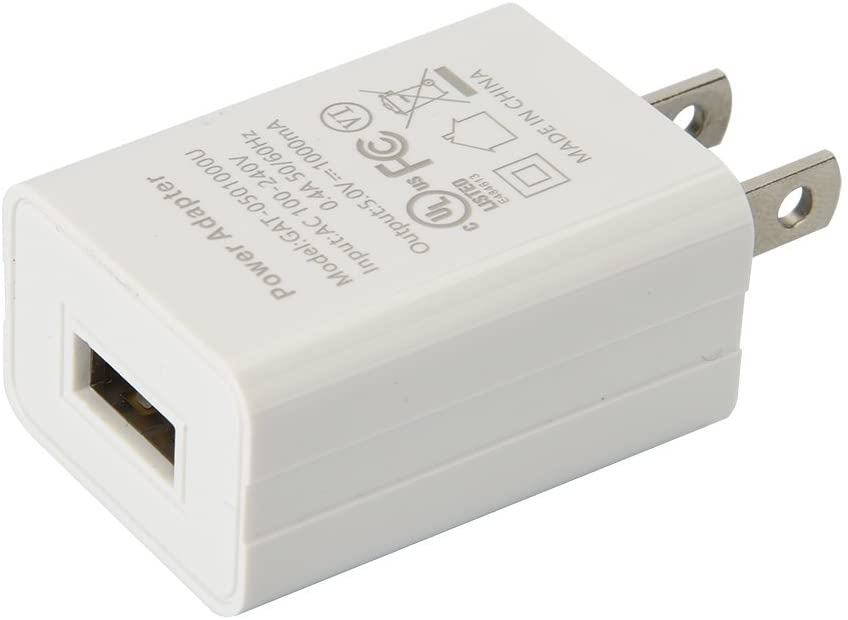
\includegraphics[width=3cm]{images/adapter.jpg}
            \caption{Power Adapter}
        \end{figure}
        \begin{flushleft}
            Power adapter will be used to power the Raspberry Pi and the ESP8266.
        \end{flushleft}
        \textbf{Specification:}
        \begin{itemize}
            \item Power: 20W
            \item Voltage: 5V
            \item Current: 2A
        \end{itemize}
        
    \subsection{Wires}
        \begin{figure}[H]
            \centering
            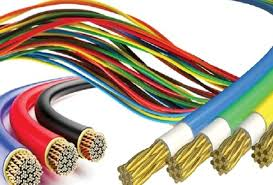
\includegraphics[width=3cm]{images/wires.jpg}
            \caption{Wires}
        \end{figure}

        \begin{flushleft}
            Wires will be used to connect the different parts 
        \end{flushleft}

\section{Required Software Stack}
    \begin{enumerate}
        \item Visual Studio Code
        \item EasyEDA
        \item OpenCV
    \end{enumerate}

    
\section{Description of Software Stack}
    \subsection{Visual Studio Code}
    \begin{flushleft}
        Visual Studio Code is a text editor that can be used to write code/text. This is a very flexible and light weight text editor. All codes 
        and text including this report has been written with Visual Studio Code. 
    \end{flushleft}
    \subsection{EasyEDA}
    \begin{flushleft}
        EasyEDA is a EDA or Electronics Design Automation tool. It can be used to design circuits and run simulations.
    \end{flushleft}
    \subsection{OpenCV}
    \begin{flushleft}
        OpenCV is a C powered image processing library. It can be used to process both still images and video stream directly from camera. We'll be using 
        it's stream analysis capabilities to find out faces in the FOV of the camera. 
    \end{flushleft}